% last updated in April 2002 by Antje Endemann
% Based on CVPR 07 and LNCS, with modifications by DAF, AZ and elle, 2008 and AA, 2010, and CC, 2011; TT, 2014; AAS, 2016

\documentclass[runningheads]{llncs}
\usepackage{graphicx}
\usepackage{amsmath,amssymb} % define this before the line numbering.
\usepackage{ruler}
\usepackage{booktabs}
\usepackage{color}
\usepackage[width=122mm,left=12mm,paperwidth=146mm,height=193mm,top=12mm,paperheight=217mm]{geometry}

\newcommand{\sz}[1]{\textcolor{blue}{\emph{//sz: #1//}}}


\begin{document}
% \renewcommand\thelinenumber{\color[rgb]{0.2,0.5,0.8}\normalfont\sffamily\scriptsize\arabic{linenumber}\color[rgb]{0,0,0}}
% \renewcommand\makeLineNumber {\hss\thelinenumber\ \hspace{6mm} \rlap{\hskip\textwidth\ \hspace{6.5mm}\thelinenumber}}
% \linenumbers
\pagestyle{headings}
\mainmatter
\def\ECCV18SubNumber{***}  % Insert your submission number here

\title{How do we get from object recognition\\ to object naming?} % Replace with your title

\titlerunning{ECCV-18 submission ID \ECCV18SubNumber}

\authorrunning{ECCV-18 submission ID \ECCV18SubNumber}

\author{Anonymous ECCV submission}
\institute{Paper ID \ECCV18SubNumber}


\maketitle

\begin{abstract}
The abstract should summarize the contents of the paper. LNCS guidelines
indicate it should be at least 70 and at most 150 words. It should be set in 9-point
font size and should be inset 1.0~cm from the right and left margins.
\dots
\keywords{We would like to encourage you to list your keywords within
the abstract section}
\end{abstract}


\section{Introduction}

Real-world objects are members of many categories. 
and speakers can typically between choose between different, more or less specific names when referring to a particular visual entity. 
For instance, the entity surrounded by the green box in Figure \ref{fig:example} is an instance of the categories \textit{female child, child, female, person, organism}, etc.\  and can be referred to with names such as e.g.\ \textit{girl, kid, cutie, daughter, person, human}.
But even though almost every task in language \& vision involves the prediction of object names (e.g. image captioning, referring expression generation, visual dialogue), hardly any research has explicitly looked at object naming, i.e.\ determining the actual word/linguistic concept that speakers would use to refer to an object (in a particular context), but see \cite{Ordonez:2016,zarriess-schlangen:2017}.
Even research in pragmatics, that traditionally deals with reference and referring expression production, has mostly focussed on attributes, rather than object names.
Recently, however, \cite{graf2016animal} have shown that object naming preferences are subject to contextual constraints and pragmatic factors: in a typical reference game set-up with images of target objects surrounded by distractor objects, speakers have been found to flexibly adjust object names depending on the context. For instance, a \textit{dalmatian} would be called \textit{dalmatian} in the context of other dogs or simply \textit{dog} when none of the distractors is also a dog.
This extends previous traditional work on concepts suggesting that the typicality of a referent determines its entry-level category (and consequently, its name) \cite{Rosch1978}.


Most research on computer vision and object recognition has somehow worked around the fact that objects can be instances of multiple, hierarchically embedded categories. 
State-of-the-art recognition models are mostly trained as classifiers on a flat of 1000 categories in ImageNet, reducing the ImageNet ontology to an inherently flat annotation scheme and treating
object labels as mutually exclusive.

On the vision side, however, there is huge body of research on object recognition, i.e.\ labeling visual objects according to a set of categories, cf.\ \cite{simonyan2014very,deng2014large,googlenet}.

\begin{figure}
\centering
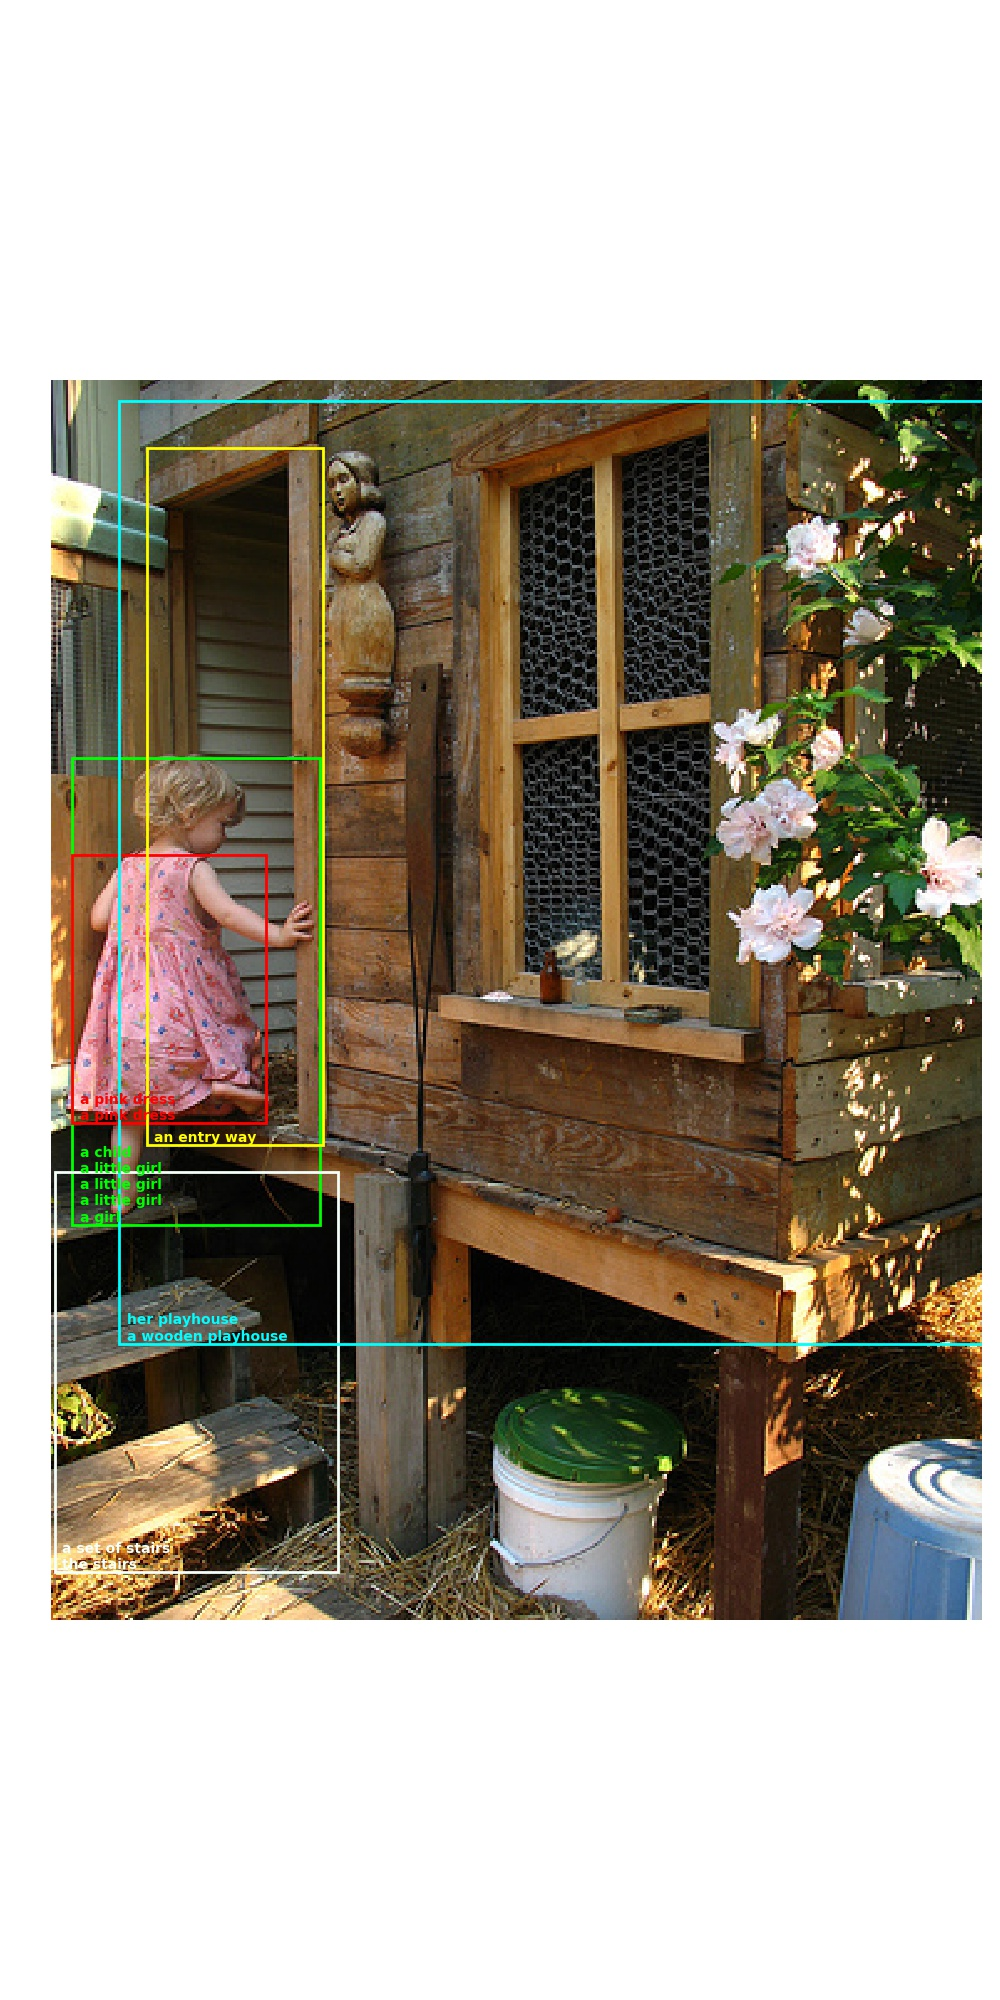
\includegraphics[height=3.5cm]{fig/flickr_1000268201_boxes}
\caption{INCLUDE MSCOCO examples}
\label{fig:example}
\end{figure}

\section{Background}

\section{Data}

\subsection{Corpora}

\paragraph{Referring Expressions}
We analyze the RefCOCO and RefCOCO+ datasets which contain referring expressions to objects in MSCOCO \cite{mscoco} images.
These data collections were performed via crowdsourcing with the ReferIt Game \cite{Kazemzadeh2014}  where two players were paired and a director needed to refer to a predetermined object to a matcher, who then selected it.
RefCOCO and RefCOCO+ contain 3 referring expressions on average per object, and overall 150K expressions for 50K objects. 
The two datasets have been collected for an (almost) identical set of objects, but in RefCOCO+, players were asked not to use location words (\textit{on the left}, etc.).
See \cite{Yu2016} for more details. 

\paragraph{Image Captions}

TODO.


\subsection{Preprocessing}

We parse referring expressions and captions with the Stanford Dependency Parser.
We extract heads/object names as follows: TODO.

\section{Names: Levels of specificity}

In this Section, we investigate whether variability of reference level can be observed in existing data sets for language \& vision.

\subsection{Using WordNet}


\cite{graf2016animal} investigate object naming with respect to reference level. They distinguish and manually annotate 3 levels: (i) sub-level (\textit{dalmatian}), (ii) basic-level (\textit{dog}), (iii) super-level (\textit{animal}).

For large-scale studies of object naming, we need to be able to automatically define the level of specificity of a name, given an ontology. 
In this Section, we investigate whether WordNet is appropriate for defining reference level. We hypothesize that the distance of a name's synset to the root node (entity) relates to its specificity.

\paragraph{Specifcity} We calculate this distance as follows: we lookup all synsets of a word and retrieve the respective paths to the root node in WordNet. 
For each word, we use the minimal path length as distance to the root node.

Table \ref{tab:specnames} shows the levels of specificity we observe for object names in the RefCoco data set.
We observe distances to the root between 2 and 17, meaning that there is a much more fine-grained distinction of levels as the three-way classification adopted by \cite{graf2016animal}.

Unfortunately, the levels of specificity predicted by WordNet do not seem to reflect linguistic intuitions, here are some problematic examples from Table \ref{tab:specnames}:

\begin{itemize}
\item elephant (10) is more specific than panda (14)? horse is less specific than elephant (10)?
\end{itemize}


\begin{table}
\centering
\setlength{\tabcolsep}{4pt}
\begin{tabular}{rrl}
\toprule
 specificity &  rel.freq. &                          top 5 names \\
\midrule
          -1 &   0.071697 &      NONE,brocolli,zeb,broc,girafe \\
           2 &   0.003898 &                         thing,things \\
           3 &   0.001182 &   object,group,set,substance,objects \\
           4 &   0.140633 &           man,person,piece,head,part \\
           5 &   0.100739 &       player,glass,baby,front,corner \\
           6 &   0.208590 &              woman,girl,kid,boy,bowl \\
           7 &   0.238708 &            guy,right,chair,lady,bear \\
           8 &   0.110613 &           horse,bus,cow,pizza,batter \\
           9 &   0.097390 &         shirt,car,bike,donut,catcher \\
          10 &   0.048368 &   elephant,couch,truck,vase,suitcase \\
          11 &   0.008828 &    motorcycle,clock,mom,dad,scissors \\
          12 &   0.002822 &  oven,airplane,suv,taxi,refrigerator \\
          13 &   0.005253 &   laptop,fridge,canoe,orioles,pigeon \\
          14 &   0.000414 &  panda,freezer,penguin,rooster,rhino \\
          15 &   0.030870 &   zebra,giraffe,zebras,giraffes,deer \\
          16 &   0.000083 &       bison,mooses,orang,elks,sambar \\
          17 &   0.000143 &           ox,cattle,gnu,mustang,orca \\
\bottomrule
\end{tabular}\caption{Levels of specificity for naming choices in RefCOCO: for each level, relative frequency and 5 most frequent names are shown}
\label{tab:specnames}
\end{table}


\clearpage

\bibliographystyle{splncs}
\bibliography{naming}
\end{document}
